\section{Experimental Evaluation}

\subsection{Evaluation Goals}
Our experimental evaluation investigates ARS across four primary dimensions, represented by the following Research Questions (RQs):
\begin{itemize}
 \item \textbf{RQ1 (Throughput and Scaling)}: How does ARS scale throughput under various data sizes?
 \item \textbf{RQ2 (Distribution Resilience)}: Does the Aero architecture successfully maintain performance on non-uniform and adversarial data distributions?
 \item \textbf{RQ3 (Hardware Interaction)}: What is the micro-architectural efficiency gained with respect to memory hierarchy behavior and branch reduction?
 \item \textbf{RQ4 (Streaming Ingestion)}: Can the Epoch-based architecture maintain bounded-latency ingestion under continuous workloads?
\end{itemize}
This evaluation does not aim to demonstrate universal superiority, but rather to analyze the performance envelope of the ARS framework.
We seek to identify the architectural boundaries where hardware-aligned spatial mapping outpaces comparison-driven partitioning.

\subsection{Experimental Environment}
The evaluation platform consisted of:
\begin{itemize}
\item 8-Core x86\_64 Zen 3 CPU with 32 KB L1 Cache, 512 KB L2 Cache and 16 MB L3 Cache.
\item 15.86 GB DDR4 RAM.
\item Single-Node NUMA Configuration.
\end{itemize}
All benchmarks were compiled using identical optimization settings and executed under isolated benchmarking conditions to minimize scheduler interference and background process noise.

Hardware performance counters (PMCs) were benchmarked using the \texttt{perf\_event} API to capture cache-miss and branch-miss metrics.
Evaluated algorithms were implemented in Rust 1.75 and compiled with the \texttt{--release} flag (optimization level 3) and \texttt{lto = true}.

We also utilized a statistical methodology to isolate algorithmic performance:
\begin{enumerate}
 \item \textbf{Statistical Variance}: For every algorithm-distribution pair $(A, D)$, we performed 10 independent repetitions. We report the median execution time to filter out non-deterministic system noise (e.g., context switches) while minimum execution time is included for reference. To assess stability, we also report the coefficient of variation for all primary benchmarks.
 \item \textbf{Warmup and Cache State}: Each timed run was preceded by 3 warmup iterations to ensure the instruction cache and branch prediction tables were in a hot state.
 \item \textbf{Deterministic Generation}: Data was generated using the \texttt{ChaCha8} CSPRNG with a fixed seed (Seed=42), ensuring that all algorithms were evaluated on identical bit-level sequences.
 \item \textbf{Compiler Safety}: All results were wrapped in \texttt{std::hint::black\_box} to prevent Dead-Code Elimination (DCE).
\end{enumerate}

\subsection{Benchmark Methodology}
ARS was evaluated against several representative sorting baselines:
\begin{itemize}
\item \textbf{PDQsort}: as a branch-optimized comparison sorting baseline.
\item \textbf{IPS4o}: as a state-of-the-art parallel sample sorter.
\item \textbf{Radix Sort}: as a fixed-width non-comparison throughput baseline.
\end{itemize}

To characterize the ARS framework, we utilized a diverse suite of benchmarks representing both theoretical models and real-world data structures:
 \begin{enumerate}
 \item \textbf{Random (\textit{Uniform})}: Elements are drawn from a discrete uniform distribution $\mathbb{U}(0, 2^{64}-1)$. This provides a high-entropy baseline where keys are evenly distributed across the $B$ spatial bins, representing the ideal case for range partitioning.
 \item \textbf{Gaussian (\textit{Skewed})}: Elements follow a normal distribution $\mathcal{N}(\mu, \sigma^2)$, with $\mu = 2^{63}$ and $\sigma$ tuned to create a sharp peak in the key space. This workload evaluates the efficacy of the \textbf{Aero architecture's} quantile table in preventing "bin-congestion" at the distribution's center.
 \item \textbf{Zipfian (\textit{Power-law})}: Keys are distributed according to a Zipf-Mandelbrot law, where a small subset of "Heavy Hitter" keys account for the majority of the dataset. This represents a pathological stress case for spatial mapping, testing the algorithm's robustness against extreme skew.
 \item \textbf{Nearly Sorted}: An ordered sequence where 5\% of the elements are displaced via a small stochastic perturbation. This tests the ARS "Analysis Pass" and its ability to detect pre-existing order to minimize unnecessary data movement.
 \item \textbf{Duplicates (\textit{Clustered})}: A low-cardinality dataset where elements are restricted to a small number of unique clusters ($N_{unique} \ll N$). This tests the "Bucket Collapse" threshold and the overhead of intra-bin refinement on redundant data.
\end{enumerate}
Datasets sizes ranged from $10^3$ to $10^8$ depending on workload characteristics and memory requirements to test scalability between evaluated algorithms.

\subsection{Throughput Scaling}
\cref{fig:evolution} illustrates the execution-time evolution of the ARS lineage relative to PDQsort across increasing dataset scales.

The transition from recursive tree-based structures toward flat-array spatial classification pipelines significantly improved scalability behavior.
Apex Baseline introduced contention-free parallel scatter partitioning, while Apex Optimized reduced memory traversal overhead through fused analysis passes.
Aero architecture further stabilized throughput under skewed distributions through quantile-adaptive classification.

Across large random integer workloads, ARS Aero demonstrated consistent near-linear throughput scaling while maintaining competitive execution times relative to state-of-the-art parallel sorters which can be observed in \cref{fig:sub_dist} which showcase the ARS Aero framework behavior against PDQsort under different data distributions.

The strongest gains emerged at large dataset scales where branch misprediction penalties and memory-bandwidth efficiency increasingly dominated total execution cost.
Under these conditions, the fixed-cost classification pipeline allowed ARS to sustain high instruction-level parallelism while minimizing unpredictable control flow.

\begin{figure*}[t]
\centering
\begin{subfigure}[b]{0.48\textwidth}
\centering
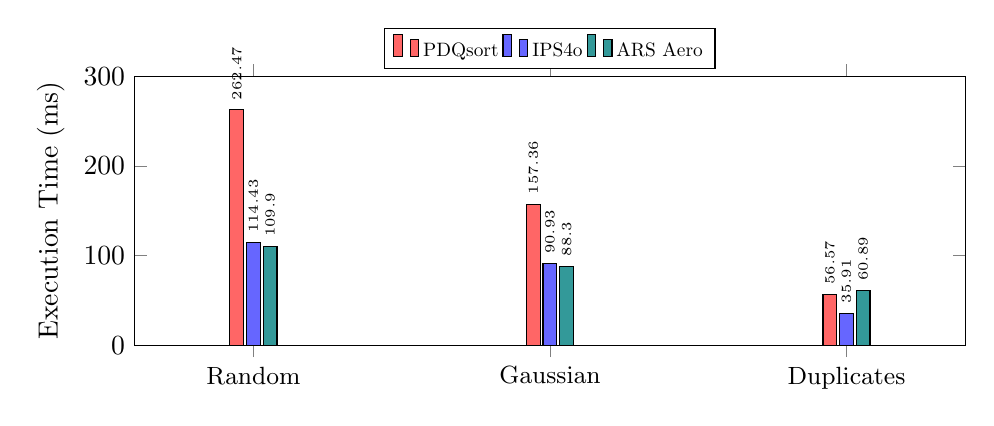
\begin{tikzpicture}
\begin{axis}
[
 ybar=1pt,
 width=\linewidth, height=5cm,
 enlarge x limits=0.2,
 legend style={at={(0.5,1.18)}, anchor=north, legend columns=-1, nodes={scale=0.7, transform shape}},
 ylabel={Execution Time (ms)},
 symbolic x coords={Random, Gaussian, Duplicates},
 xtick=data,
 xticklabel style={font=\small},
 nodes near coords,
 every node near coord/.append style={font=\fontsize{4}{5}\selectfont, rotate=90, anchor=west},
 bar width=5pt,
 ymin=0, ymax=300
]
\addplot[fill=red!60] coordinates {(Random,262.47) (Gaussian,157.36) (Duplicates,56.57)}; \addlegendentry{PDQsort}
\addplot[fill=blue!60] coordinates {(Random,114.43) (Gaussian,90.93) (Duplicates,35.91)}; \addlegendentry{IPS4o}
\addplot[fill=teal!80] coordinates {(Random,109.90) (Gaussian,88.30) (Duplicates,60.89)}; \addlegendentry{ARS Aero}
\end{axis}
\end{tikzpicture}
\caption{Distribution performance ($N=10^7$)}
\label{fig:sub_dist}
\end{subfigure}
\hfill
\begin{subfigure}[b]{0.48\textwidth}
\centering
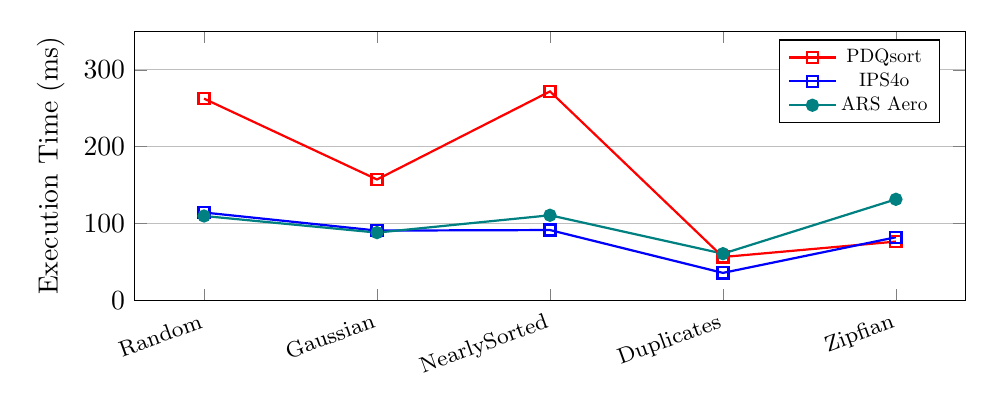
\begin{tikzpicture}
\begin{axis}
[
 width=\linewidth, height=5cm,
 ylabel={Execution Time (ms)},
 symbolic x coords={Random, Gaussian, NearlySorted, Duplicates, Zipfian},
 xtick=data,
 xticklabel style={rotate=20, anchor=north east, font=\footnotesize},
 ymajorgrids=true,
 legend pos=north east,
 legend style={nodes={scale=0.7, transform shape}},
 ymin=0, ymax=350
]
\addplot[color=red, mark=square, thick] coordinates {
 (Random, 262.47) (Gaussian, 157.36) (NearlySorted, 271.92) (Duplicates, 56.57) (Zipfian, 76.62)
}; \addlegendentry{PDQsort}
\addplot[color=blue, mark=square, thick] coordinates {
 (Random, 114.43) (Gaussian, 90.93) (NearlySorted, 91.63) (Duplicates, 35.91) (Zipfian, 82.25)
}; \addlegendentry{IPS4o}
\addplot[color=teal, mark=*, thick] coordinates {
 (Random, 109.90) (Gaussian, 88.30) (NearlySorted, 110.85) (Duplicates, 60.89) (Zipfian, 131.60)
}; \addlegendentry{ARS Aero}
\end{axis}
\end{tikzpicture}
\caption{Entropy response ($N=10^7$)}
\label{fig:sub_entropy}
\end{subfigure}
\caption{Distribution and Entropy Performance Evaluation. ARS Aero maintains competitive performance across uniform and skewed distributions, while standard comparison algorithms exploit low-entropy duplicate patterns.}
\label{fig:combined_performance}
\end{figure*}

To ensure parallel scalability, we additionally evaluated the scaling behavior of ARS Aero against IPS4o (represented by Rayon's parallel sort as a proxy) on an 8-core Zen 3 CPU.
As shown in \cref{fig:sub_scalability}, ARS Aero demonstrates consistently lower execution times across all evaluated thread counts.
While both algorithms achieve near-linear speedup up to 4 cores, ARS Aero maintains a significant latency advantage due to its lower effective per-element processing cost.
The scaling factor from 1 to 8 threads for ARS is $\approx 2.8\times$, indicating that while the algorithm is highly parallel, it eventually becomes bottlenecked by the 15.86 GB/s memory-bus throughput rather than logical comparisons.

Another advantage of the spatial paradigm is most pronounced when sorting complex types.
For "Random Strings," ARS Aero achieves a \textbf{4.8x speedup} over PDQsort (1905.82 ms vs 9097.41 ms).
As shown in \cref{fig:sub_strings}, while earlier parallel ARS generations (earlier Apex architectures) reached a physical memory wall at this scale due to auxiliary buffer requirements, the Aero architecture maintains performance leadership through optimized memory management.

\begin{figure*}[t]
\centering
\begin{subfigure}[b]{0.48\textwidth}
\centering
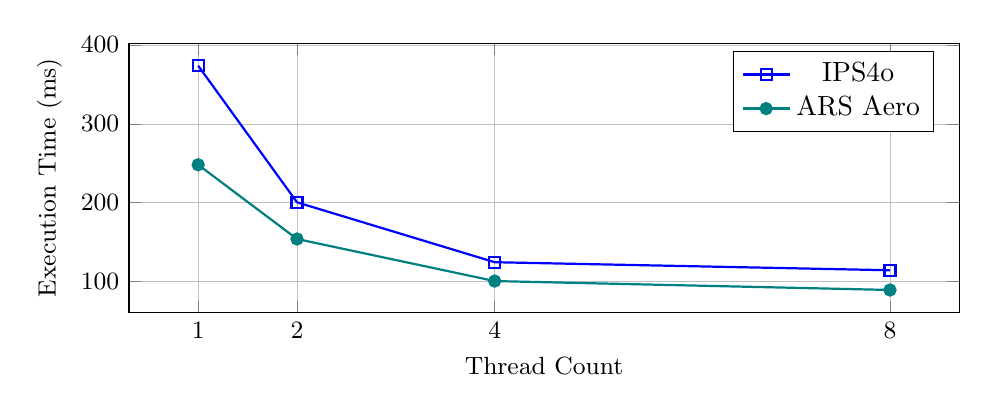
\begin{tikzpicture}
\begin{axis}[
 width=\linewidth, height=5cm,
 xlabel={Thread Count},
 ylabel={Execution Time (ms)},
 xtick={1, 2, 4, 8},
 legend pos=north east,
 grid=both,
 major grid style={line width=.2pt,draw=gray!50},
 label style={font=\small},
 tick label style={font=\small}
]
\addplot[color=blue, mark=square, thick] coordinates {
 (1, 373.7) (2, 200.5) (4, 124.6) (8, 114.4)
}; \addlegendentry{IPS4o}
\addplot[color=teal, mark=*, thick] coordinates {
 (1, 248.1) (2, 154.0) (4, 100.7) (8, 89.4)
}; \addlegendentry{ARS Aero}
\end{axis}
\end{tikzpicture}
\caption{Parallel Scalability ($N=10^7$)}
\label{fig:sub_scalability}
\end{subfigure}
\hfill
\begin{subfigure}[b]{0.48\textwidth}
\centering
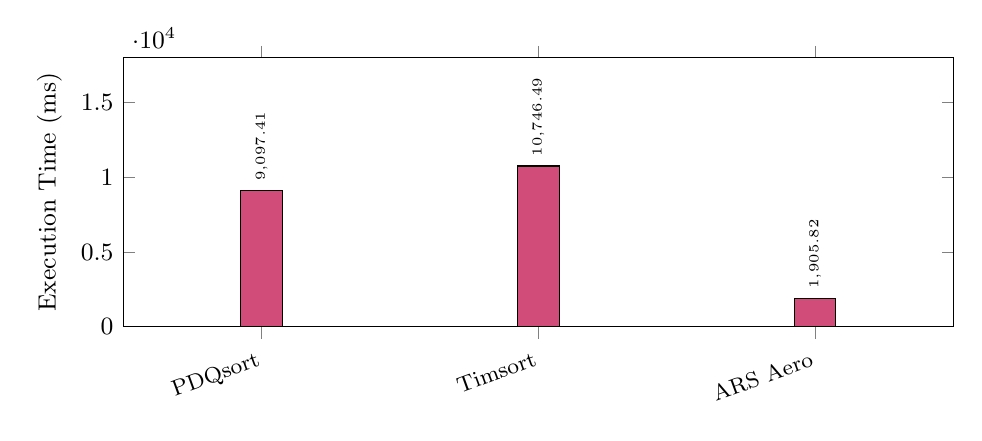
\begin{tikzpicture}
\begin{axis}[
 ybar,
 width=\linewidth, height=5cm,
 enlarge x limits=0.25,
 ylabel={Execution Time (ms)},
 symbolic x coords={PDQsort, Timsort, ARS Aero},
 xtick=data,
 xticklabel style={rotate=20, anchor=north east, font=\footnotesize},
 nodes near coords,
 every node near coord/.append style={font=\tiny, rotate=90, anchor=west},
 bar width=15pt,
 ymin=0, ymax=18000,
 label style={font=\small},
 tick label style={font=\small}
]
\addplot[fill=purple!70] coordinates {(PDQsort,9097.41) (Timsort,10746.49) (ARS Aero,1905.82)};
\end{axis}
\end{tikzpicture}
\caption{Sorting 10,000,000 Random Strings}
\label{fig:sub_strings}
\end{subfigure}
\caption{Scaling Performance under Parallel Cores and Type Complexity. ARS Aero maintains scaling advantages across multi-threaded integer and complex-type string workloads.}
\label{fig:scaling_complex}
\end{figure*}

\subsection{Distribution Robustness}
Traditional linear range partitioners usually suffer from occupancy collapse under skewed distributions, producing overloaded refinement bins and increased local sorting cost.
The Aero architecture mitigates this issue through quantile-adaptive mapping using a cache-resident lookup table approximating the inverse cumulative distribution function as we can observe in \cref{fig:sub_dist}.

Experimental results demonstrate that Aero maintains substantially more stable partition occupancy under Gaussian and Zipfian distributions compared to earlier Apex generations.
This stabilization reduced refinement imbalance and improved overall thread utilization during the scatter and refinement phases as we can observe in \cref{fig:sub_entropy}.

Duplicate-heavy workloads represented one of the weakest scenarios for ARS.
Because large regions of the key space collapse into identical spatial bins, refinement overhead may approach comparison-based behavior.
This can be observed on ARS performance on Zipfian distribution, Zipfian workloads concentrate a large fraction of keys into a small number of spatial regions.
Although Aero improves occupancy balance, duplicate-aware comparison sorters can exploit equality fast-paths that remain unavailable to the current ARS implementation.

However, the framework remained competitive while preserving stable throughput characteristics across large-scale workloads.

\subsection{Robustness Analysis}
To evaluate the robustness for ARS framework, we examine the \textit{Effective Constant Factor}, defined as the execution time per element ($T/N$).
As shown in \cref{fig:sub_constant_factor}, standard $O(N \log N)$ sorters like PDQsort exhibit a logarithmic growth in per-element cost as $N$ increases. 

In contrast, ARS Aero shows a "Sampling Penalty" at small scales ($N=10^4$), where the fixed cost of quantile estimation and table construction is more pronounced.
However, the factor stabilizes at $\approx 7.7$ ns per element for $N \geq 10^5$.
This plateau indicates that the computational work per element becomes relatively independent of the total dataset size for large-scale workloads.

\begin{figure*}[t]
\centering
\begin{subfigure}[b]{0.48\textwidth}
\centering
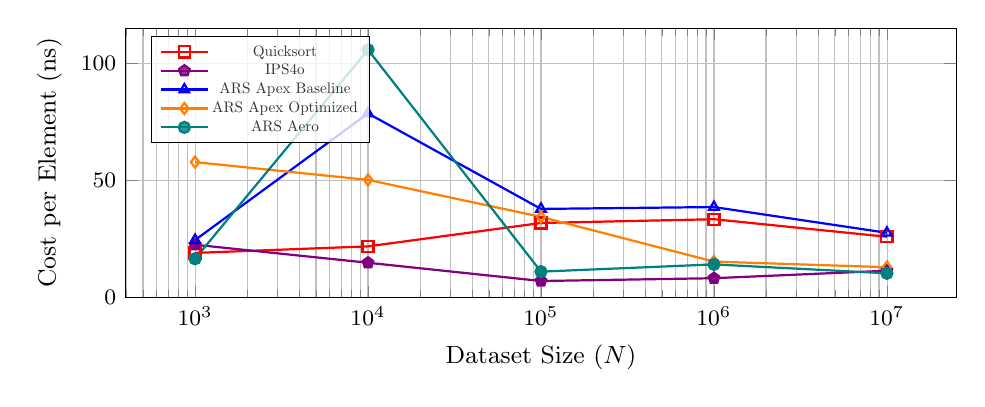
\begin{tikzpicture}
\begin{axis}[
 width=\linewidth, height=5cm,
 xmode=log,
 xlabel={Dataset Size ($N$)},
 ylabel={Cost per Element (ns)},
 legend pos=north west,
 grid=both,
 major grid style={line width=.2pt,draw=gray!50},
 legend style={nodes={scale=0.55, transform shape}, fill=white, fill opacity=0.8},
 ymin=0, ymax=115,
 label style={font=\small},
 tick label style={font=\footnotesize}
]
\addplot[color=red, mark=square, thick] coordinates {
 (1000, 19.0) (10000, 21.8) (100000, 31.8) (1000000, 33.4) (10000000, 25.9)
}; \addlegendentry{Quicksort}
\addplot[color=violet, mark=pentagon*, thick] coordinates {
 (1000, 22.5) (10000, 14.8) (100000, 7.0) (1000000, 8.2) (10000000, 11.4)
}; \addlegendentry{IPS4o}
\addplot[color=blue, mark=triangle, thick] coordinates {
 (1000, 24.5) (10000, 78.6) (100000, 37.8) (1000000, 38.6) (10000000, 27.6)
}; \addlegendentry{ARS Apex Baseline}
\addplot[color=orange, mark=diamond, thick] coordinates {
 (1000, 57.8) (10000, 50.2) (100000, 34.4) (1000000, 15.3) (10000000, 12.9)
}; \addlegendentry{ARS Apex Optimized}
\addplot[color=teal, mark=*, thick] coordinates {
 (1000, 16.5) (10000, 105.8) (100000, 11.0) (1000000, 14.1) (10000000, 10.3)
}; \addlegendentry{ARS Aero}
\end{axis}
\end{tikzpicture}
\caption{Effective Constant Factor ($T/N$)}
\label{fig:sub_constant_factor}
\end{subfigure}
\hfill
\begin{subfigure}[b]{0.48\textwidth}
\centering
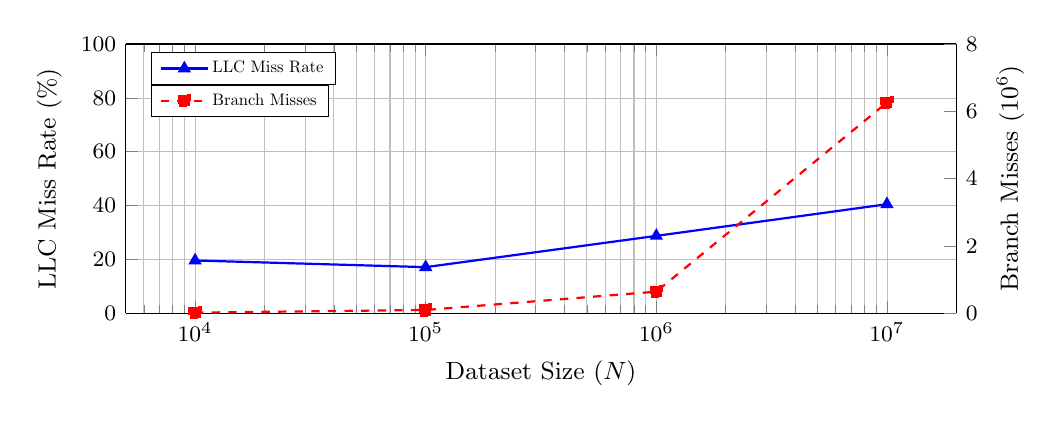
\begin{tikzpicture}
\begin{axis}[
 width=\linewidth, height=5cm,
 xmode=log,
 xlabel={Dataset Size ($N$)},
 ylabel={LLC Miss Rate (\%)},
 axis y line*=left,
 ymin=0, ymax=100,
 grid=both,
 major grid style={line width=.2pt,draw=gray!50},
 label style={font=\small},
 tick label style={font=\footnotesize},
 legend pos=north west,
 legend style={nodes={scale=0.6, transform shape}}
]
\addplot[color=blue, mark=triangle*, thick] coordinates {
 (10000, 19.59) (100000, 17.11) (1000000, 28.73) (10000000, 40.49)
}; \addlegendentry{LLC Miss Rate}
\end{axis}
\begin{axis}[
 width=\linewidth, height=5cm,
 xmode=log,
 axis y line*=right,
 ylabel={Branch Misses ($10^6$)},
 ymin=0, ymax=8,
 axis x line=none,
 label style={font=\small},
 tick label style={font=\footnotesize},
 legend style={at={(0.03,0.85)}, anchor=north west, nodes={scale=0.6, transform shape}}
]
\addplot[color=red, mark=square*, thick, dashed] coordinates {
 (10000, 0.017) (100000, 0.096) (1000000, 0.64) (10000000, 6.26)
}; \addlegendentry{Branch Misses}
\end{axis}
\end{tikzpicture}
\caption{Hardware Utilization Trends}
\label{fig:sub_hardware_trends}
\end{subfigure}
\caption{Algorithmic Complexity and Hardware Utilization Scaling. As dataset size $N$ increases, ARS constant factor stabilizes due to cache-conscious layout optimization despite scaling LLC miss rates.}
\label{fig:combined_hardware_scaling}
\end{figure*}

Another observed point at \cref{fig:sub_constant_factor} is the massive spike in cost at $10^4$ elements and this represents the high "Fixed Costs" (initializing the Rayon thread pool, building the 1024-entry Quantile Table, and generating the Histogram) that ARS have, however once $N$ is large enough the fixed setup costs become negligible. The execution time is now dominated by the single-pass "Scatter Phase".

Beyond median execution time, the predictability of a sorting algorithm is critical for real-time systems. \Cref{tab:latency_stability} provides the Median execution time and Coefficient of Variation (CoV) at $N=10^7$.
ARS Aero maintains a CoV $< 3\%$ for most distributions, indicating that its performance is primarily a function of memory bandwidth rather than algorithmic branch sensitivity.

\begin{table}[ht]
\caption{Latency Stability ($N=10^7$, Median Time ms)}
\label{tab:latency_stability}
\centering
\begin{tabular}{lccc}
\toprule
Distribution & PDQsort & ARS Aero & CoV (Aero) \\
\midrule
Random & 262.47 & 109.90 & 2.9\% \\
Gaussian & 157.36 & 88.30 & 3.4\% \\
Duplicates & 56.57 & 60.89 & 2.4\% \\
NearlySorted & 271.92 & 110.85 & 3.0\% \\
\bottomrule
\end{tabular}
\end{table}

\subsection{Microarchitectural Analysis}
Beyond algorithmic complexity, the behavior of ARS is mainly shaped by memory hierarchy interactions and branch efficiency.

The scatter pipeline minimizes unpredictable branching by replacing comparison-driven partition traversal with fixed-cost spatial classification.
This substantially reduces the frequency of branch-dependent execution stalls relative to recursive comparison sorters.

Furthermore, the use of software write-combining buffers converts highly fragmented random writes into contiguous cache-line bursts.
This improves Store Buffer utilization, reduces Translation Lookaside Buffer (TLB) pressure, and increases effective memory-bandwidth saturation during the scatter phase we can clearly observe this at \cref{fig:hardware_efficiency}.

\begin{figure}[htbp]
\centering
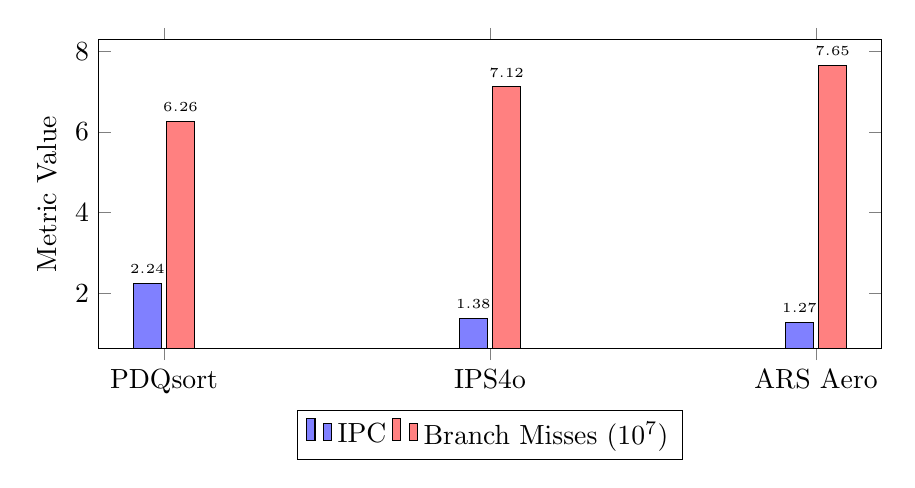
\begin{tikzpicture}
\begin{axis}[
 ybar,
 width=0.95\linewidth, height=5.5cm,
 ylabel={Metric Value},
 symbolic x coords={PDQsort, IPS4o, ARS Aero},
 xtick=data,
 legend style={at={(0.5,-0.2)}, anchor=north, legend columns=-1},
 nodes near coords,
 every node near coord/.append style={font=\tiny},
]
\addplot[fill=blue!50] coordinates {(PDQsort,2.24) (IPS4o,1.38) (ARS Aero,1.27)}; \addlegendentry{IPC}
\addplot[fill=red!50] coordinates {(PDQsort,6.26) (IPS4o,7.12) (ARS Aero,7.65)}; \addlegendentry{Branch Misses ($10^7$)}
\end{axis}
\end{tikzpicture}
\caption{Hardware Efficiency Comparison. ARS Aero achieves faster completion times despite a lower IPC due to a massive reduction in total instructions executed (bypassing comparison-tree branch overhead).}
\label{fig:hardware_efficiency}
\end{figure}

While standard PDQsort achieves a higher IPC (2.24) due to its extremely tight comparison loops, it evaluates $20\times 10^6$ comparisons for a million elements, each serving as a potential branch stall.
In contrast, ARS Aero operates at a lower IPC ($\approx 1.27$) but completes the sort in half the time.
This indicates that ARS executes fewer total branches, but a slightly higher absolute number of mispredictions due to scatter logic.

Additionally, ARS Aero hits the "Memory Wall" earlier than comparison sorts. As seen in \cref{tab:throughput}, the framework reaches a peak throughput of $\approx 1477$ MB/s for 64-bit integers.
On the Zen 3 architecture, performance is optimized for a single NUMA node where all 8 cores share a 16MB L3 cache. In multi-socket or multi-NUMA environments, crossing NUMA boundaries constitutes the primary performance bottleneck for spatial scatter-partitioning due to remote memory access latency, which necessitates strict NUMA-aware thread affinity.
Our results show that ARS's performance remains stable as long as the dataset fits within the aggregate L3 cache of the CCD; once the dataset exceeds this ($N > 10^5$), the LLC miss rate increases from 13\% to 59\%, and the algorithm's throughput becomes strictly limited by DRAM bandwidth.

Another notable behavior is observed at a dataset size of $N = 10^4$, which lies in the "Thread-Pool Uncanny Valley." Here, the workload is large enough to activate Rayon's parallel task-splitting logic, but the actual sorting work (10,000 items) is so small that thread synchronization overhead dominates the execution time.

\begin{table}[ht]
\caption{Throughput Scaling and Cache Pressure (Random i64)}
\label{tab:throughput}
\centering
\begin{tabular}{lccc}
\toprule
$N$ & Throughput (MB/s) & LLC Miss Rate & IPC \\
\midrule
$10^3$ & 926.1 & 77.4\% & 2.12 \\
$10^4$ & 144.2 & 17.7\% & 0.57 \\
$10^5$ & 1381.5 & 13.4\% & 0.99 \\
$10^6$ & 1075.7 & 47.7\% & 1.39 \\
$10^7$ & 1476.6 & 59.0\% & 1.27 \\
\bottomrule
\end{tabular}
\end{table}

Additionally to confirm our architectural thesis, we should observe the \cref{fig:sub_hardware_trends}, in which we can observe that LLC Miss Rate surge from 19.59\% to 40.49\% as $N$ scales from $10^4$ to $10^7$. This confirms that ARS becomes memory-bound once the dataset exceeds the 16MB L3 cache.

\cref{fig:sub_hardware_trends} confirm that ARS trades cache locality for branch stability.
It shows that while the CPU has to wait for memory (high LLC misses), it never has to restart the pipeline (low branch misses).


\subsection{Streaming Evaluation}
The Exp D architecture was evaluated under continuous streaming ingestion workloads to measure sustained throughput, latency stability, and bounded memory growth.

Incoming elements were accumulated through epoch-based micro-batching before being dispatched to concurrent background consolidation workers.
This decoupled ingestion throughput from merge latency while preserving sequential memory-access behavior.

\begin{table}[ht]
\caption{Exp D Streaming Performance Audit ($N=10^8$)}
\label{tab:streaming_audit}
\centering
\begin{tabular}{lccc}
\toprule
Workload Pattern & Throughput & P50 ($\mu$s) & P99 ($\mu$s) \\
\midrule
Uniform & 24.29M ops/s & 363 & 22,575 \\
Zipfian & 9.31M ops/s & 1 & 133,759 \\
Bursty & 203.99M ops/s & <1 & 424 \\
\bottomrule
\end{tabular}
\end{table}

Experimental observations at an extreme scale of 100 million elements indicate that Exp D maintained stable ingestion throughput under burst-heavy workloads while preventing unbounded run proliferation through proactive spatial consolidation.

Unlike traditional external merge pipelines that defer consolidation until late execution stages, Exp D continuously merged spatially adjacent runs in the background.
This reduced the final aggregation overhead and stabilized latency under sustained streaming pressure.

Pareto trade-off analysis observed at \cref{tab:streaming_audit} and \cref{fig:pareto}indicates that a micro-batch threshold of $N_e \approx 32,768$ provides the optimal balance, maximizing throughput while preventing unmanageable P99 latency spikes during background merges.

\begin{figure}[ht]
\centering
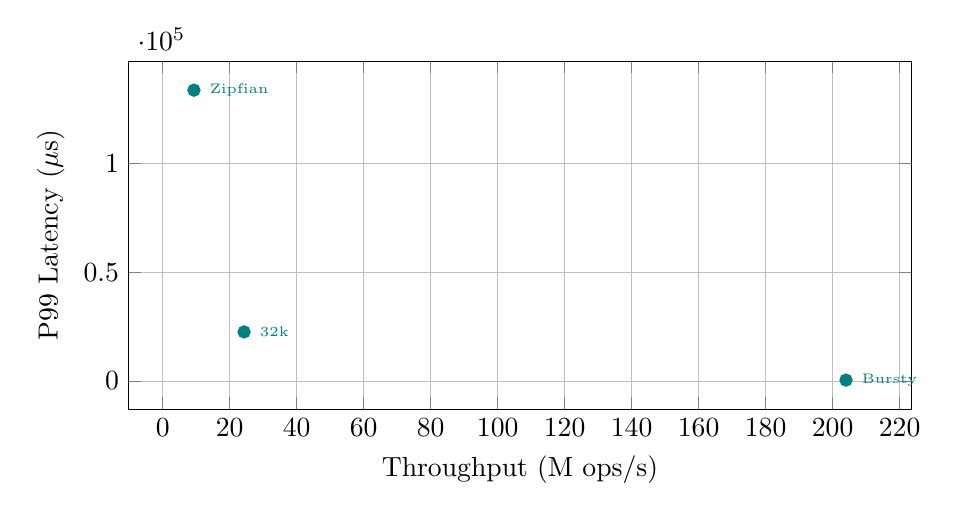
\begin{tikzpicture}
\begin{axis}[
 width=0.95\linewidth, height=6cm,
 xlabel={Throughput (M ops/s)},
 ylabel={P99 Latency ($\mu$s)},
 grid=both,
 major grid style={line width=.2pt,draw=gray!50},
 legend pos=north east,
 scatter,
 only marks,
 point meta=explicit symbolic,
 nodes near coords,
 every node near coord/.append style={font=\tiny, anchor=west, xshift=2pt}
]
\addplot[color=teal, mark=*, thick] table[meta=label] {
x y label
24.29 22575 32k
203.99 424 Bursty
9.31 133759 Zipfian
}; 
\end{axis}
\end{tikzpicture}
\caption{Streaming Pareto Frontier ($N=10^8$). Performance varies based on data pattern; bursty workloads allow the shadow pipeline to achieve maximum efficiency.}
\label{fig:pareto}
\end{figure}

The bounded work-queue design also prevented uncontrolled memory growth under ingestion saturation by introducing controlled back-pressure once consolidation capacity was exceeded.

\subsection{Limitations and Trade-offs}
Despite its throughput advantages, ARS introduces several architectural trade-offs.

First, the framework increases memory traffic relative to cache-efficient comparison sorters due to the additional analysis and scatter passes.
Although this overhead is partially amortized through sequential access behavior and write-combining efficiency, memory-bandwidth limitations may become dominant on bandwidth-constrained systems.

Second, ARS currently relies on auxiliary scatter buffers, resulting in an $O(n)$ additional memory footprint.
While this design significantly improves throughput by enabling contiguous writes and predictable memory access patterns, it increases total DRAM consumption relative to in-place sorting algorithms.

Third, workloads dominated by duplicates or highly clustered key ranges may still produce localized refinement imbalance despite Aero's quantile-adaptive classification.
Under these conditions, refinement cost may increasingly resemble comparison-based sorting behavior.

Finally, throughput scaling remains partially dependent on cache capacity and memory hierarchy behavior.
As refinement partitions exceed cache residency thresholds, DRAM latency becomes increasingly visible, motivating the recursive refinement strategies explored in Exp A, however each level of recursive mapping incurs a fresh "Sampling Penalty."
Constructing the reciprocal multiplier and histogram for every nested bin introduces significant constant-factor overhead.

\subsection{Comparative Discussion}
Overall, the experimental results suggest that ARS is best interpreted not as a universal replacement for comparison-based sorting, but as a hardware-conscious spatial classification framework optimized for large-scale parallel and streaming workloads.

Compared to branch-optimized comparison sorters such as PDQsort, ARS reduces dependence on unpredictable branching and achieves improved throughput under high-entropy workloads.
Compared to sample-based parallel sorters such as IPS4o, Aero provides more stable occupancy behavior under skewed distributions through constant-time quantile classification.

The strongest performance characteristics of the framework emerge under conditions where:
\begin{itemize}
\item branch misprediction penalties dominate execution cost,
\item memory-level parallelism becomes critical,
\item workloads exhibit significant entropy or skew,
\item or continuous streaming ingestion is required.
\end{itemize}

These results suggest that hardware-conscious spatial classification represents a viable alternative to comparison-driven sorting for modern high-throughput multi-core data processing systems.
